%% Version
\def\CurrentVersionMain{\textit{V2.0}}

%LTeX: language=de-DE 

%% Dokumentenklasse und Präambel
\documentclass[12pt,a4paper,oneside,bibliography=totocnumbered,toc=listofnumbered]{scrbook}
\usepackage[english,ngerman,naustrian]{babel}
\usepackage{./packages/WissensArbeitenFHWels}
\usepackage{./packages/WissensArbeitenFHWels-FrontseitenDE} 
\usepackage[autostyle=true,german=quotes]{csquotes} 
\usepackage{float} 
\usepackage{microtype}

\usepackage{listings}



%% Einstellungen
\ColoredLinks{No}	
\Style{FHWels}				
\BibStyle{FHWelsNumericBrackets}	
\addbibresource{Bibliography.bib}	
\graphicspath{{./Grafik/}}
\TabContent{1.4cm}	
\setlength {\marginparwidth }{2cm}

%% Beginn der ARBEIT
\begin{document}
    \selectlanguage{naustrian}		

    %% Titelseite
    \clearpage
    \frontmatter								
    \pagenumbering{Roman}	
    \begin{titlepage}
	\vspace*{-17mm}
	%% ------------------------------------------
    %% Bildheader 
    %% ------------------------------------------

    %% Bild
	\begin{center}
		\begin{figure}[h]
			\centering
			
\includegraphics[width=9.5cm]{Grafik/FH.png}
		\end{figure}
		
        %% Studiengang
		\vspace{6mm}
	  	{\textsc{\Large Studiengang}}
		\vskip 2mm
	  	{\Large Automatisierungstechnik}
		\vskip 0mm
		\rule{15cm}{0.3mm}

    %% ------------------------------------------
    %% Mittelteil innerhalb der Trennstriche
    %% ------------------------------------------

        %% Fach
        \vskip 7mm
        \textbf{\large Masterprojekt 2}
        
        %% Art
		\vskip 0mm
		Projekt-Bericht

        %% Semester
		\vskip 0mm
        Wintersemester 2023

        %% Titel 
		\vskip 10mm
		\textbf{\LARGE{Entwicklerdokumentation: Productboard}}

        %% Foto
		\vskip 8mm
        \begin{figure}[h]
			\centering
            %% Erstes Bild
			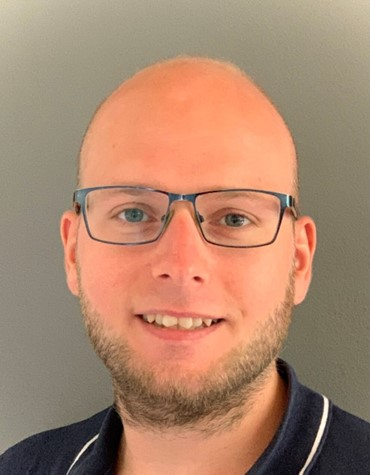
\includegraphics[width=3cm]{Grafik/userPic.jpg}
		\end{figure}
		
        %% 1.Autor
		\vskip 5mm
        \textbf{\large {Dominik Frühwirth / S2110564009}}
        
		
        %% Datum
        \vskip 6mm
        Abgabedatum:
        \vskip 0mm
	  	03.März 2023
	  
        %% ------------------------------------------
        %% Unterteil
        %% ------------------------------------------

        %% Betreuer
	  	\vspace{5mm}
	  	\rule{15cm}{0.3mm}
	  	\vskip 5mm
	  	Betreuung des Masterprojekts durch
	  	\vskip 0mm
        Dr. Georg Hackenberg
		
	\end{center}
\end{titlepage}

    %% Inhaltsverzeichnis
    \clearpage
    \tableofcontents

    %% Einleitung
    \clearpage
    \mainmatter
    %LTeX: language=de-DE
\chapter{Einleitung}

Die Software mit dem vorläufigen Namen ''Productboard'' [siehe Abb. \ref{fig: productview} auf S.~\pageref{fig: productview}] soll Stakeholder bei der Entwicklung neuer Produkte unterstützen oder als Hilfsmittel zur Erforschung von Produktentwicklungsprozessen dienen. Ähnlich der Webplattform ''GitHub\footnote{https://github.com}'' können auch hier Arbeitsergebnisse hochgeladen werden um diese zu versionieren und zu verwalten. Im Unterschied zu GitHub liegt der Fokus hierbei jedoch nicht auf Sourcecode, sondern auf 3D-CAD Modellen.

\begin{figure}[h]
    \centering
    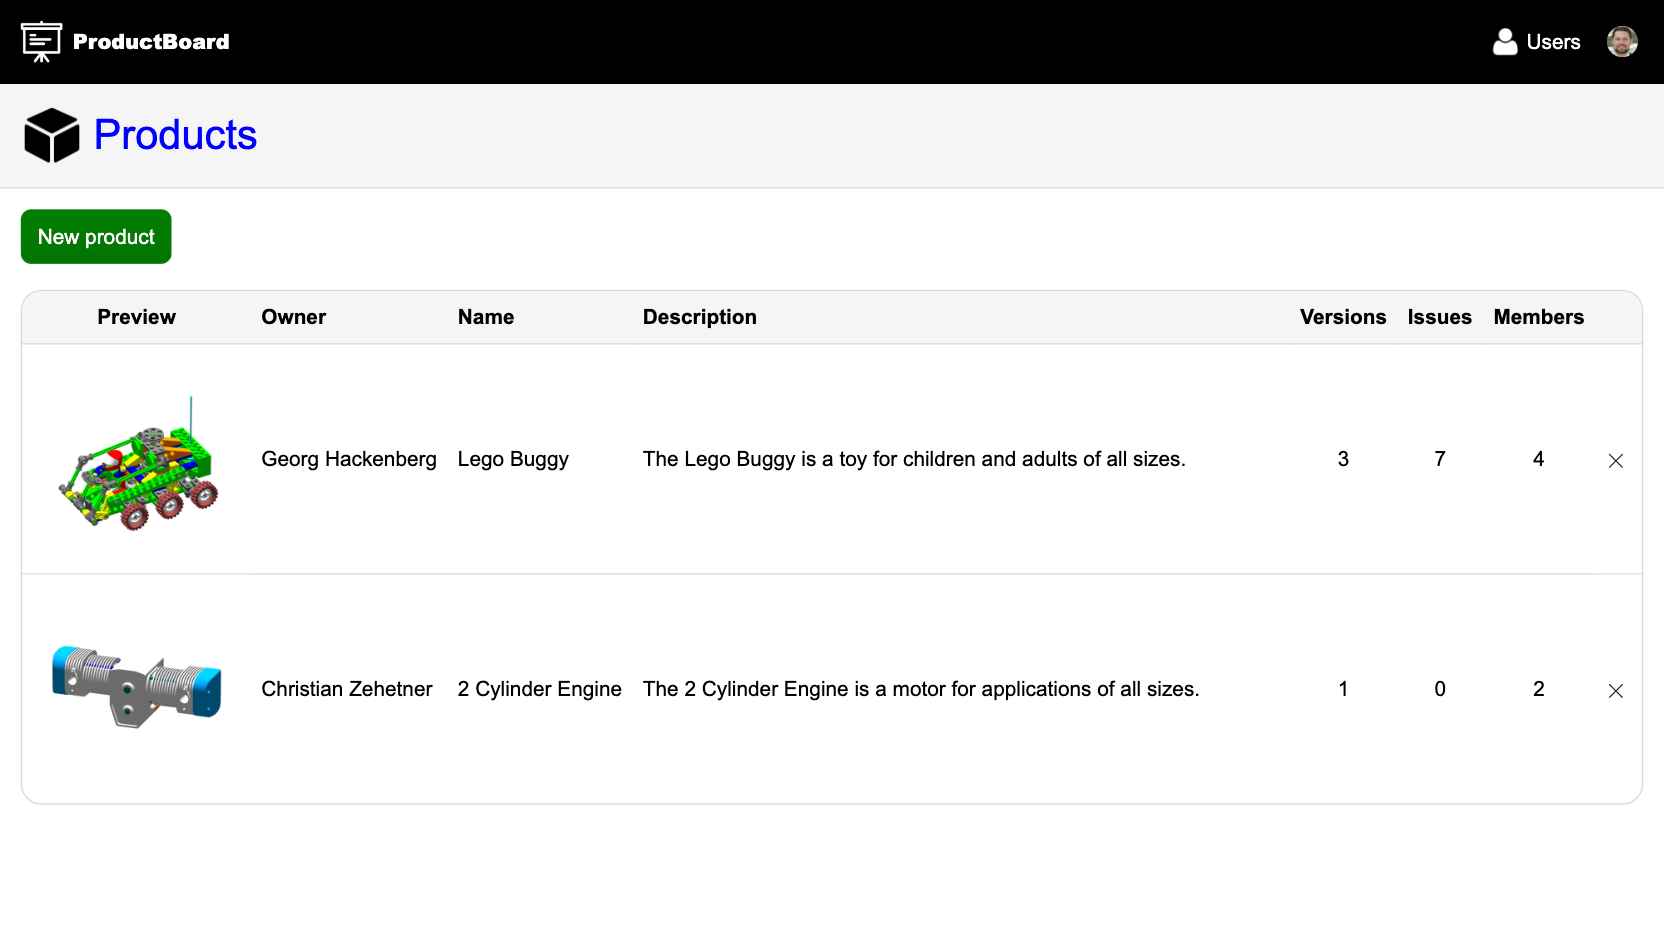
\includegraphics[width=1\textwidth]{productview.png}
    \caption{Product View}
    \label{fig: productview}
\end{figure} 

Jedes Produkt führt auf die jeweilige Produktseite, [siehe Abb. \ref{fig: versionview} auf S.~\pageref{fig: versionview}] auf der Projektmanagementtools angeboten werden, die in Tabs unterteilt sind:
\begin{itemize}
	\item Versions: In diesem Tab können über den ''New version'' Button neue Versionen hinzugefügt werden. Diese werden dann in der Listenansicht angezeigt und können durch Anklicken groß in der 3D-Ansicht auf der rechten Seite betrachtet werden.
	\item Issues: Dient zum Hinzufügen neuer Issues. Diese werden dann als Liste angezeigt und können nach offenen und geschlossenen Issues gefiltert werden. Hinter jedem Issue befindet sich ein Kommunikationskanal, wo die Issues in Textform oder durch Audioaufnahmen besprochen werden können.
	\item Milestones: Dient zum Erstellen von Sprints. Diese Sprints können dann mit Issues befüllt werden. Ein Burn-Down-Chart zeigt den Fortschritt des jeweiligen Sprints an.
	\item Members: Hier kann definiert werden, welche User der Plattform das jeweilige Produkt sehen können und welche Rechte sie haben das Produkt zu bearbeiten.
	\item Settings: Hier können der Produktname und die Produktbeschreibung nachträglich geändert werden.
\end{itemize}

\begin{figure}[h]
    \centering
    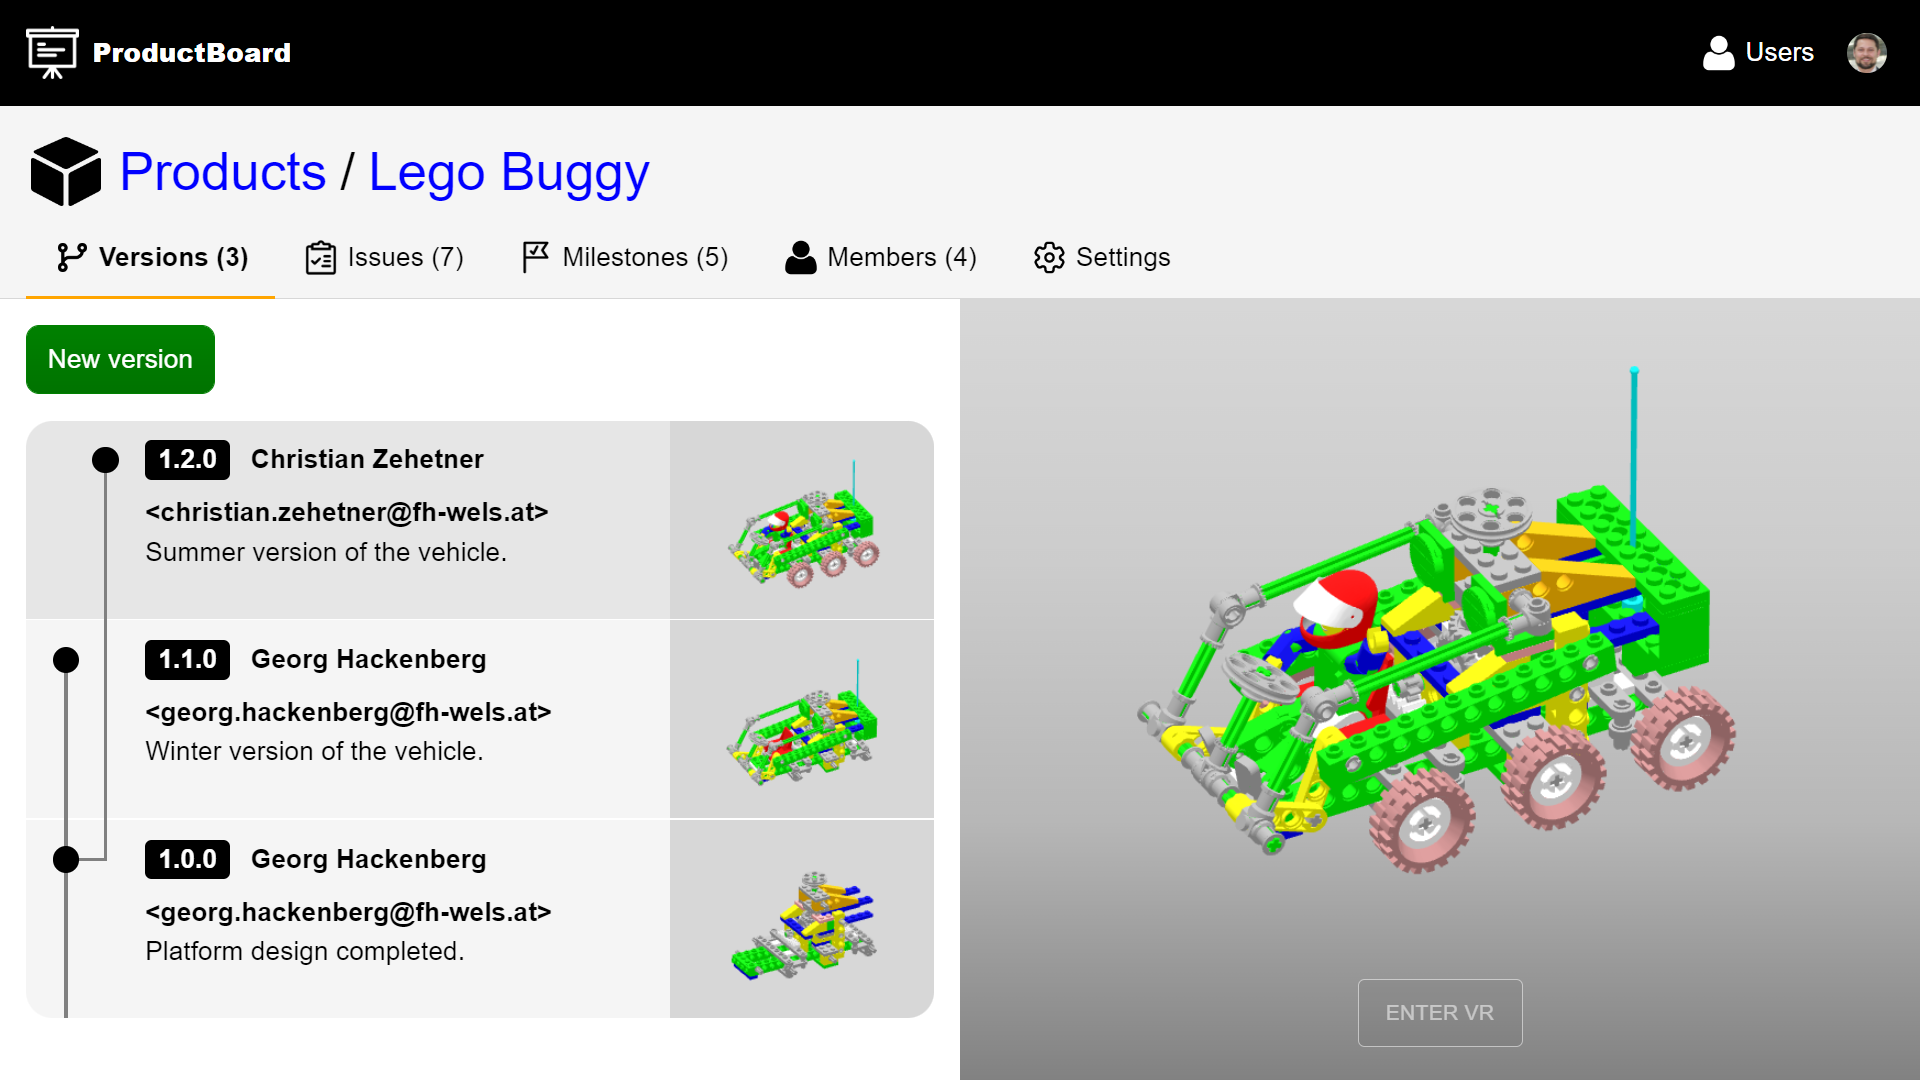
\includegraphics[width=1\textwidth]{versionview.png}
    \caption{Version View}
    \label{fig: versionview}
\end{figure}

Auf der rechten Seite wird das 3D-CAD Modell der ausgewählten Version angezeigt. Das Modell kann mit der Maus bewegt und gedreht werden. Mit dem Mausrad lässt sich die Zoomstufe einstellen. Die Applikation berücksichtigt auch kleinere Bildschirmgrößen, sodass bei kleineren Displays unten eine Tableiste erscheint, mit der zwischen der Tabellenansicht und der Modellansicht gewechselt werden kann. 

    %% Hauptteil			
    %LTeX: language=de-DE
\chapter{Architektur}

Bei der Applikation handelt es sich um eine Fullstack Webapp mit den Hauptkomponenten Gateway, Frontend, Backend, Datenmodell (Common) und der Datenbank. Die gesamte Anwendung ist in der Programmiersprache ''TypeScript\footnote{https://www.typescriptlang.org}'' implementiert. Die nachfolgende Abbildung [siehe Abb. \ref{fig: architektur} auf S.~\pageref{fig: architektur}] zeigt, wie die verschiedenen Pakete aufeinander aufbauen.
\begin{figure}[h]
    \centering
    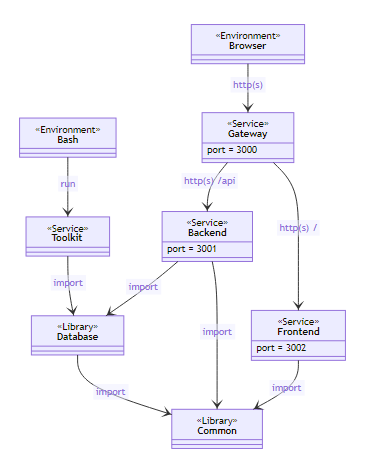
\includegraphics[width=0.8\textwidth]{architecture.png}
    \caption{Architektur}
    \label{fig: architektur}
\end{figure}

    %LTeX: language=de-DE
\chapter{Datenmodell}
Das Datenmodell (Common) wird von den Packages Frontend, Backend und Database importiert. Im Common Package wird der Vertrag erstellt, welche Daten zwischen den Packages ausgetauscht werden dürfen und wie diese Daten beschaffen sein müssen.
Die nachfolgende Abbildung [siehe Abb. \ref{fig: datamodel} auf S.~\pageref{fig: datamodel}] zeigt das Datenmodell der Applikation:
\begin{figure}[h]
    \centering
    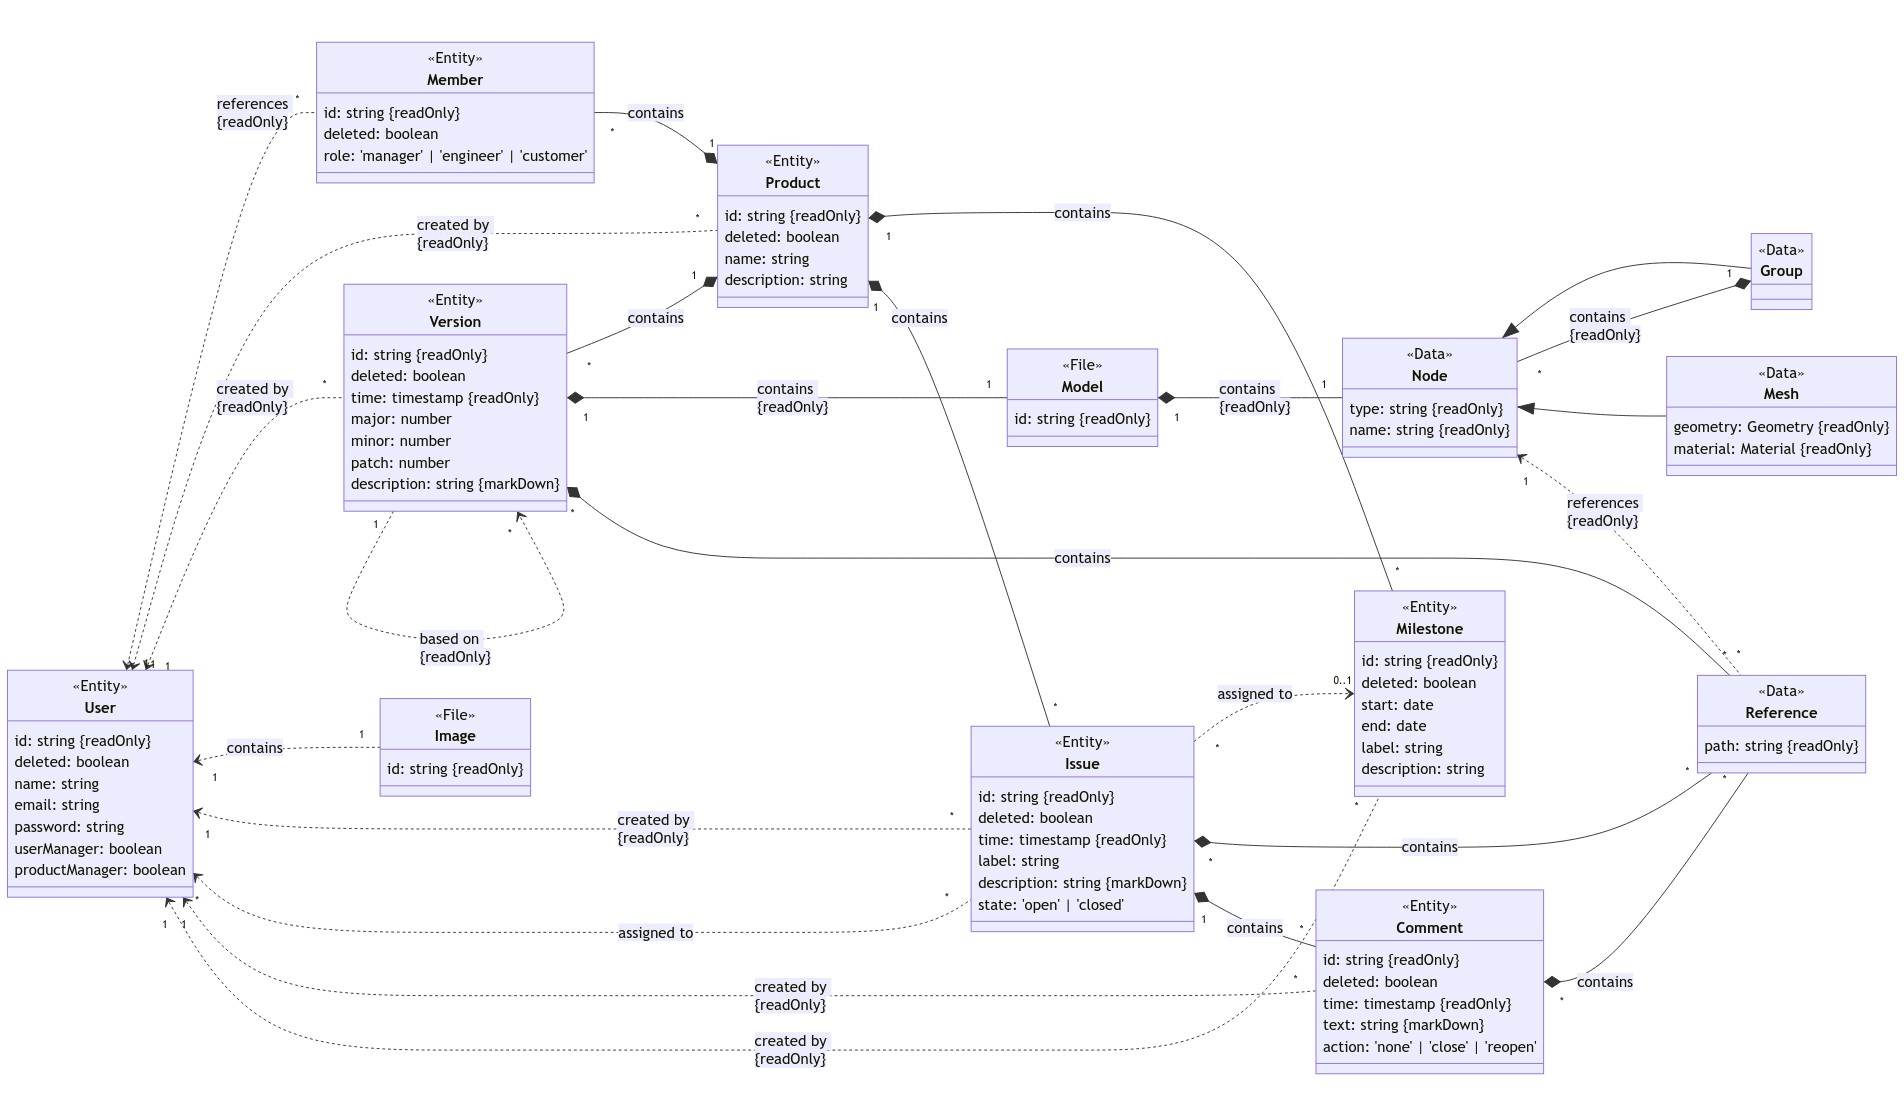
\includegraphics[width=1\textwidth]{datamodel.png}
    \caption{Datenmodell}
    \label{fig: datamodel}
\end{figure}

Die Implementierungen der Entities sind im Verzeichnis ''packages/common/src/data'' zu finden. Als Beispiel für die Implementierung wird, ein Ausschnitt vom Code für die ''ProduktEntity'' herangezogen [siehe Abb. \ref{fig: productdata} auf S.~\pageref{fig: productdata}]. In Zeile 1 wird das Modul für die Swagger-Dokumentation [siehe Abb. \ref{fig: swagger} auf S.~\pageref{fig: swagger}] eingebunden, welche alle Endpunkte der API übersichtlich auflistet. Mit dem Befehl ''@ApiProperty()'' werden dann die jeweiligen Einträge zur Swagger-Dokumentation\footnote{https://swagger.io}  hinzugefügt. Wie jedes Entity im Datenmodell, besteht auch das Product Entity aus drei Klassen: ''ProductUpdateData'', ''ProductAddData'', ''Product'', die hierarchisch aufeinander aufbauen. Sie definieren welche Daten später über die API geändert werden können, welche Daten beim Hinzufügen generiert werden und elementare Eigenschaften der Entity. 

\begin{figure}[h]
    \centering
    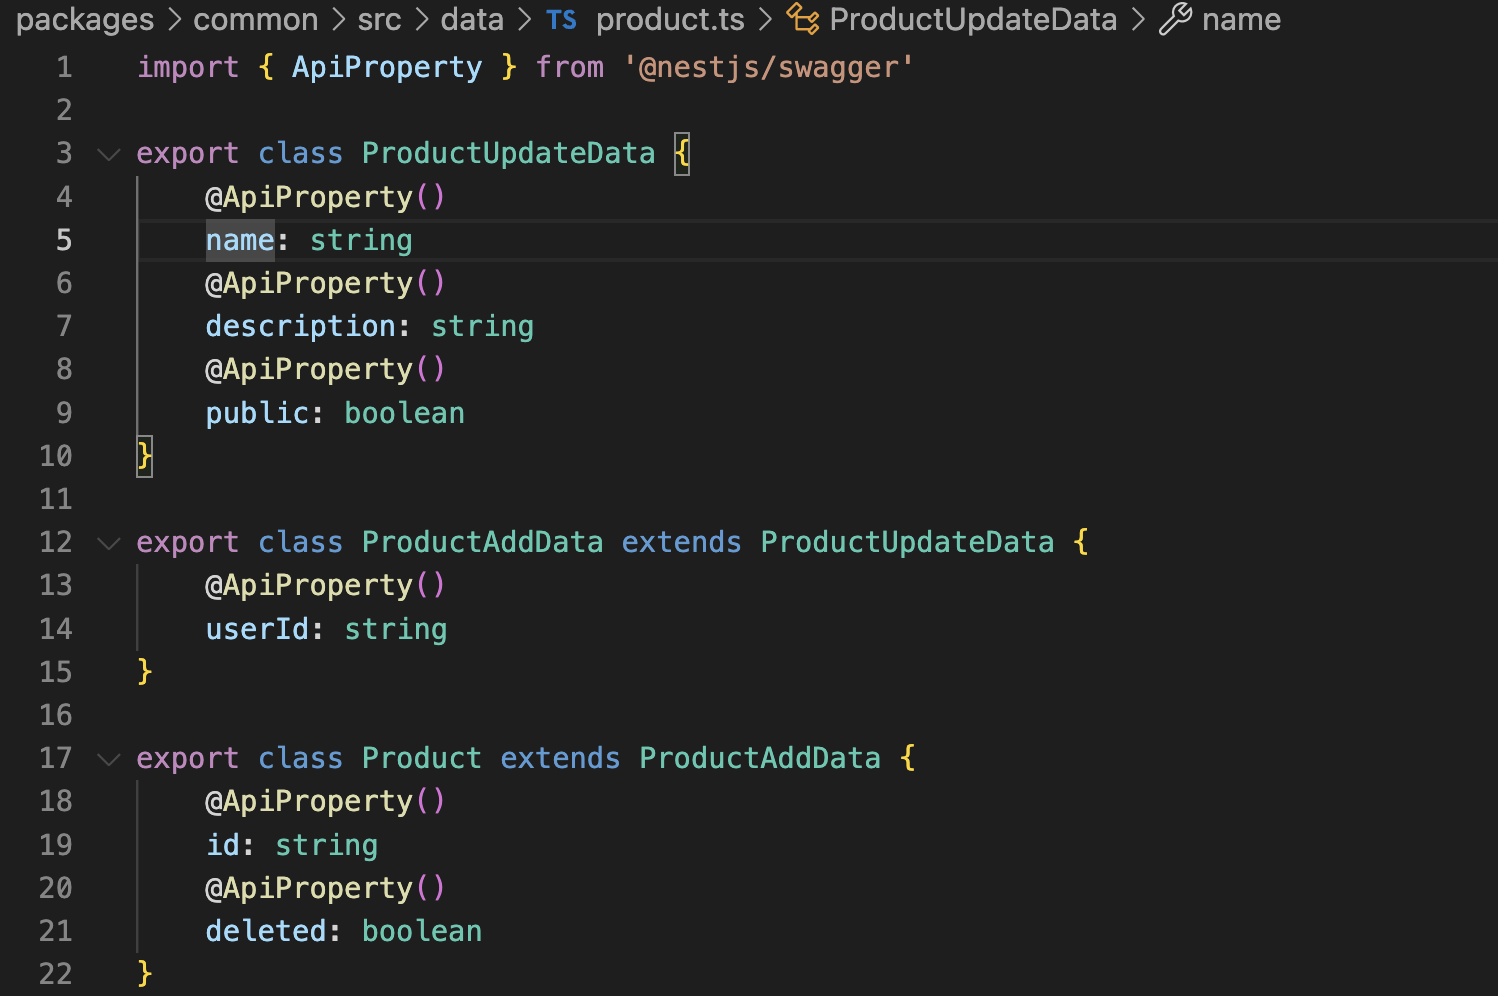
\includegraphics[width=1\textwidth]{productdata.png}
    \caption{Produkt Entity}
    \label{fig: productdata}
\end{figure}

\begin{figure}[h]
    \centering
    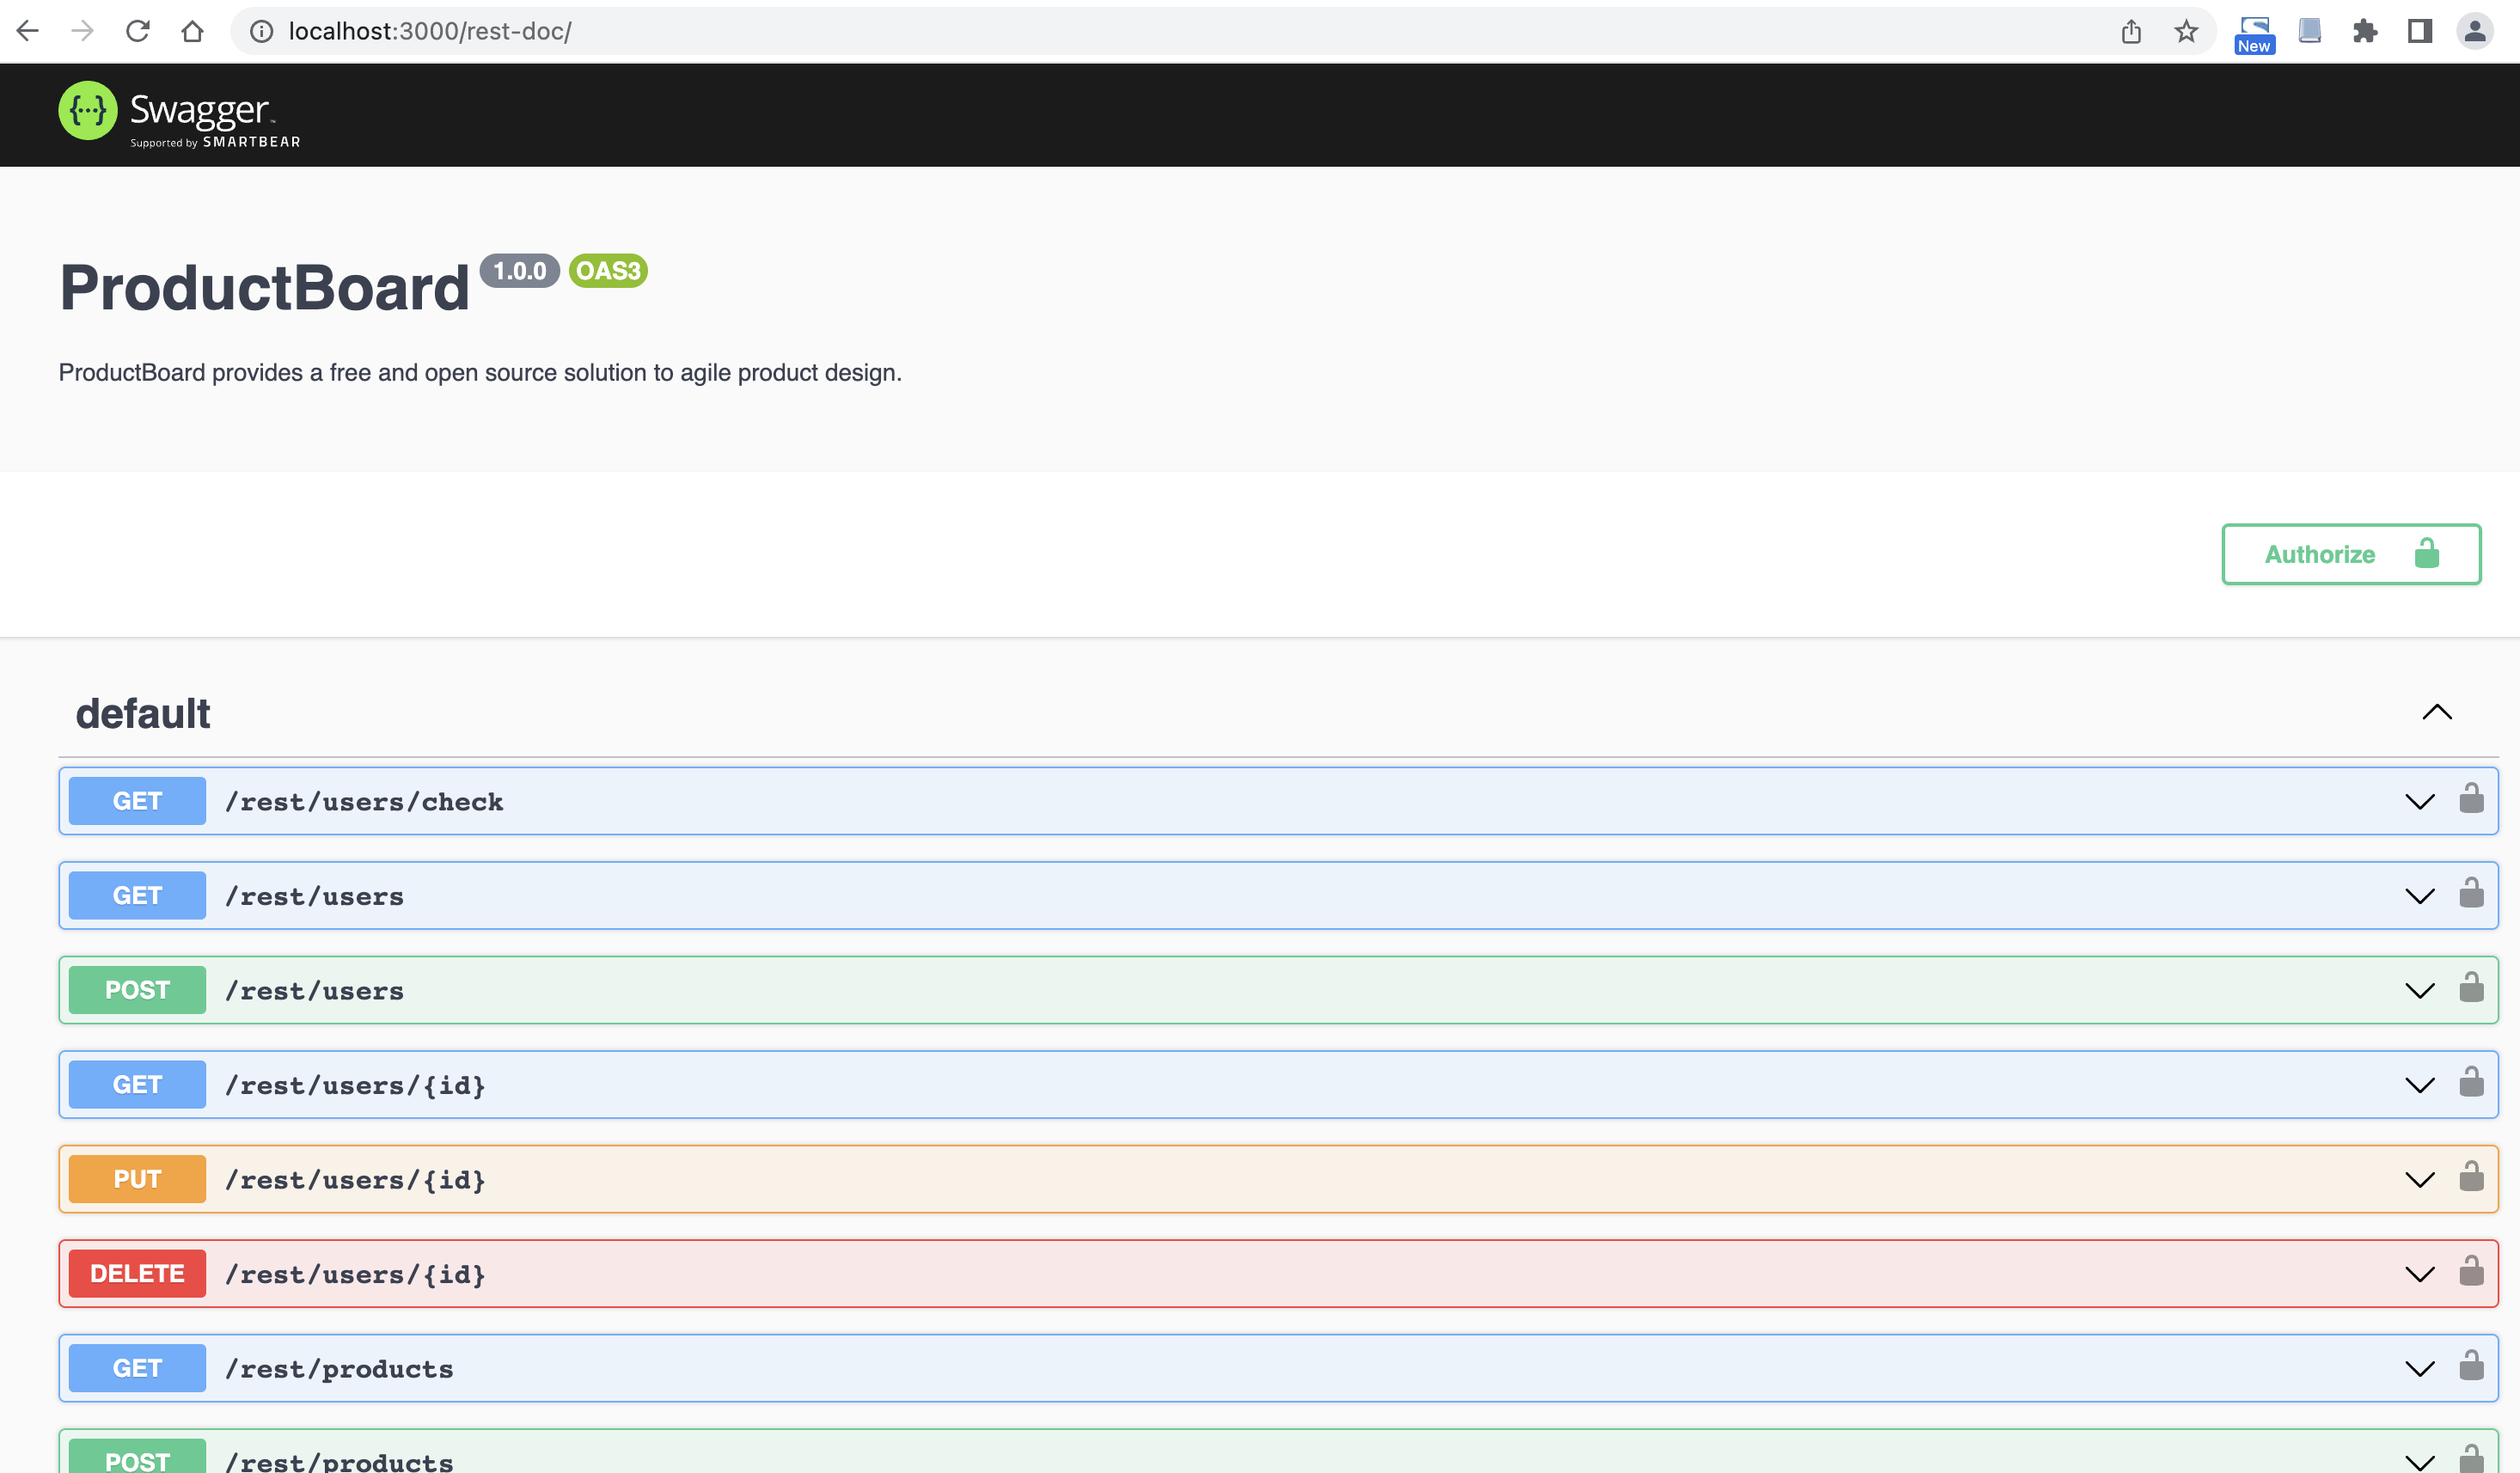
\includegraphics[width=1\textwidth]{swagger.png}
    \caption{Swagger Dokumentation}
    \label{fig: swagger}
\end{figure}
    %LTeX: language=de-DE
\chapter{Gateway}
Das Gateway lässt die Applikation nach außen hin auf einen einzigen Port laufen. In Wirklichkeit laufen aber mehrere HTTP-Server, wie Frontend, Backend, Broker, zur selben Zeit auf verschiedenen Ports. Das Gateway startet auf Port 3000 und verteilt dann die Anfragen auf die verschiedenen Ports der anderen HTTP-Server.
Die ''main.ts'' des Gateways ist im Projektverzeichnis unter ''packages/gateway/src'' zu finden.
Der dazugehörige Codeausschnitt [siehe Abb. \ref{fig: gateway} auf S.~\pageref{fig: gateway}] zeigt wie das Gateway implementiert ist. 

\begin{figure}[h]
    \centering
    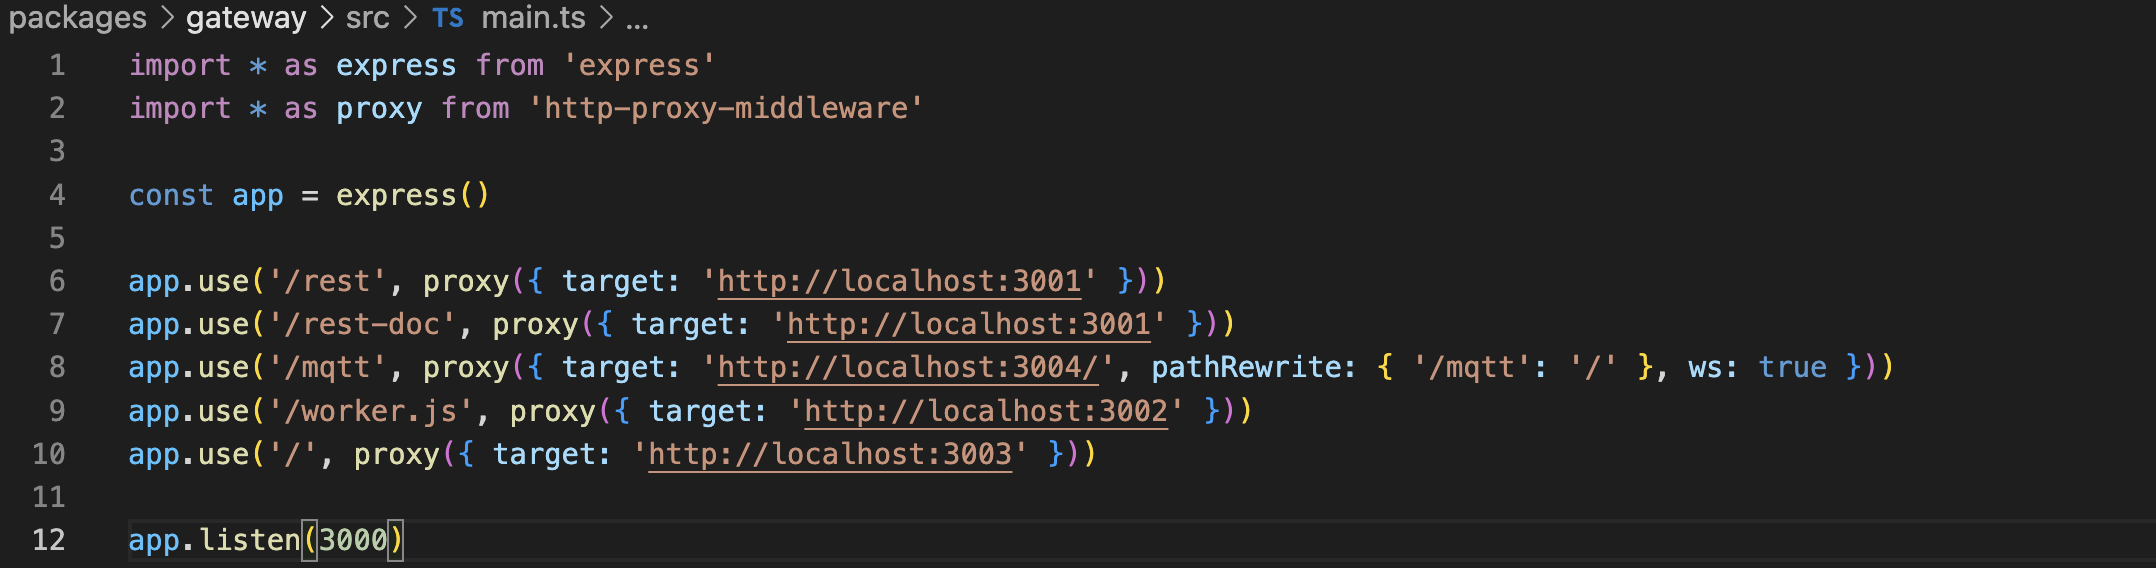
\includegraphics[width=1\textwidth]{gateway.png}
    \caption{Gateway}
    \label{fig: gateway}
\end{figure}
    %LTeX: language=de-DE
\chapter{Frontend}
Das Frontend ist jener Teil, der im Browser sichtbar ist und dient als Schnittstelle zwischen dem Anwender und den Daten. Es kann mithilfe einer Programmierschnittstelle (API) auf diese Daten zugreifen, um diese verändern oder anzeigen zu können. Für die Implementierung wurde die Bibliothek ''React\footnote{https://reactjs.org}'' verwendet. Im ''frontend/src'' Verzeichnis liegen drei Unterverzeichnisse: ''images'': Beinhaltet alle Abbildungen, die im Frontend angezeigt werden, ''scripts'': Beinhaltet den TypeScript und HTML Code zum Aufbau des Frontends, ''styles'': Beinhaltet die CSS Files für das Styling der Oberflächen. 

\section{Main.tsx}
Der Einstiegspunkt der React-App liegt im Verzeichnis ''frontend/src/scripts''. Das dort liegende File ''main.tsx'' [siehe Abb. \ref{fig: frontendmain} auf S.~\pageref{fig: frontendmain}] rendert das ''<Root/>'' Element der App, in dem dann die verschiedenen Views über den Router hineingerendert werden. Dafür wird zuerst ein ''root'' Element erstellt, dass an den ''body'' angefügt wird. Die ''ReactDom.render(element,container)'' Methode rendert dann das Element in das vorher erzeugte ''div'' Tag. Das Element, dass der ''render'' Methode mitgegeben wird beinhaltet zusätzlich noch den ''<Auth0Provider/>'' für das Anmelden über verschiedene Plattformen wie zum Beispiel dem Microsoft Account und den ''<BrowserRouter>'' für das Routing innerhalb des Frontends. Das ''<Helmet>'' Tag wird wie der ''<head>'' tag einer HTML Datei verwendet um Metadaten, wie das App-Icon, angeben zu können.

\begin{figure}[h]
    \centering
    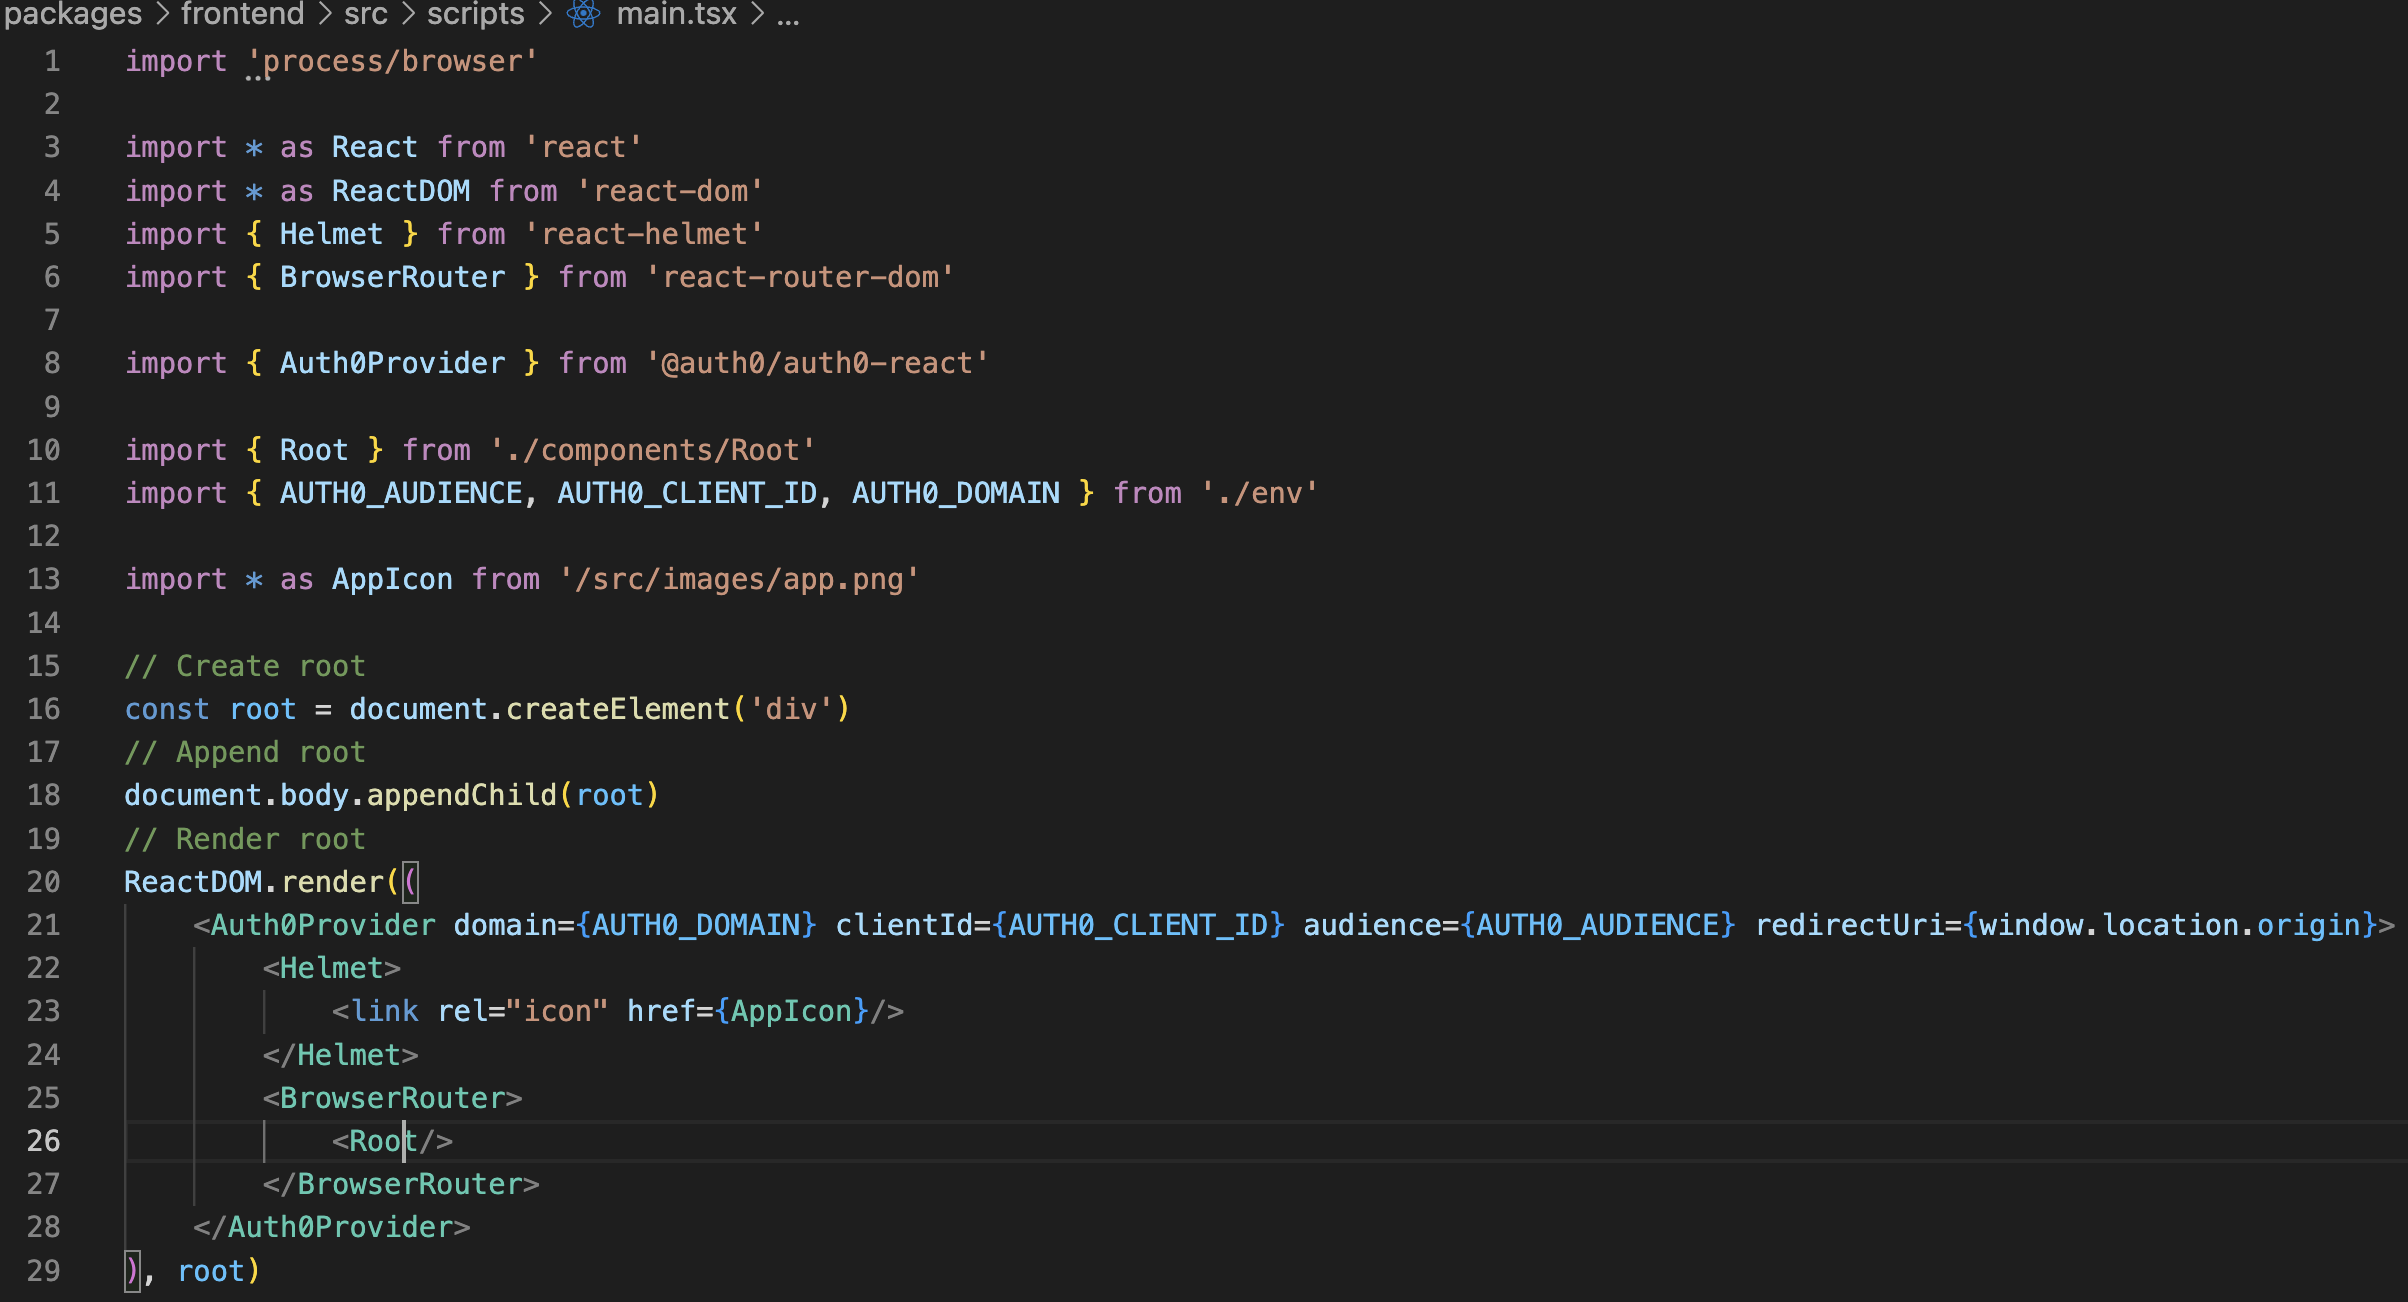
\includegraphics[width=1\textwidth]{frontendmain.png}
    \caption{main.tsx}
    \label{fig: frontendmain}
\end{figure}

\section{Root.tsx}
Im Verzeichnis ''frontend/src/scripts/components'' liegt die Datei ''Root.tsx''. Dabei handelt es sich um jene Komponente, die mit dem ''<Root/>'' tag in der ''main.tsx'' eingebunden wird. Die ''Root.tsx'' kümmert sich um das Authentifizieren des Users mit Auth0\footnote{https://auth0.com}, stellt für den User und die Produktversion eine globale Variable (useContext) bereit und definiert die Routen innerhalb der App. Bei den Routen wird definiert bei welcher URL im Browser, welche View gerendert werden soll.

\section{Aufbau der Views}
Im Verzeichnis ''frontend/src/scripts/components/views'' liegen alle Views, die mithilfe des React-Routers gerendert werden können. Dabei ist der Code jeder View ähnlich strukturiert: Ganz oben kommen die Imports und darunter wird die View in einer Arrowfunktion aufgebaut und exportiert. Dafür gibt es in jeder View folgende Bereiche:
\begin{itemize}
    \item REFERENCES: Hier wird der ''useRef'' Hook verwendet, um von einer funktionalen Komponente direkt auf ein DOM Element zugreifen zu können. So kann zum Beispiel auf einen Textinput zugegriffen werden um darauf den Fokus zu setzen.
    \item PARAMS: Sind Variablen, die aus der aktuellen URL entnommen werden, wie zum Beispiel die Produkt ID. 
	\item CONTEXTS: Globale States, die über das ganze Frontend hinweg ausgelesen und überschrieben werden können. So ist über alle Tabs hinweg der aktive User bekannt oder die eingestellte Version eines Produkts kann in allen Tabs angezeigt werden ohne diese neu einstellen zu müssen.
	\item INITIAL STATES: Hier werden Daten geholt, die bereits im Cache des Frontends vorhanden sind.
	\item STATES: Sind als ''useState'' realisiert und verhalten sich wie Properties, die gelesen und mit einer Methode beschrieben werden können. Ändert sich ein State, so wird der aktuelle Tab neu gerendert.
	\item EFFECTS: Hier werden die Daten mit ''useEffect(effect, deps)'' aus dem Backend geholt, wenn sich ein Wert in der jeweiligen DependencyList (deps) ändert. Eine leere DependencyList bedeutet, dass der ''useEffect'' beim Besuchen der Seite einmalig aufgerufen wird. 
	\item FUNCTIONS: In diesem Bereich sind Funktionen definiert, die anderswo im selben File aufgerufen werden können. Wie zum Beispiel das Löschen eines Produkts über einen Button.
	\item CONSTANTS: Definiert konstante Strukturen, wie zum Beispiel Tabellenspalten, die variabel mit den geladenen Daten befüllt werden können.
	\item RETURN: Hier ist der Rückgabewert der Arrowfunktion. In einem Return wird ein HTML Tag zurückgegeben, der verschiedene Kindelemente beinhalten kann. Der Inhalt der aktuellen Route wird dann von der ''ReactDOM.render'' Methode von der main.tsx auf dem Bildschirm dargestellt.
\end{itemize}
React bietet den Vorteil, dass sich eigene Komponenten erstellen lassen, die dann in anderen Komponenten wiederverwendet werden können. So wurden für die verschiedensten Anwendungsfälle bereits Komponenten erstellt, die in anderen Komponenten verwendet werden können. Es findet sich zum Beispiel im Verzeichnis ''frontend/src/scripts/components/widgets'' das File ''Table.tsx'', welches bei fast jeder View zum Einsatz kommt um die geladenen Daten tabellarisch anzeigen zu können. Diese Komponenten sind nach Kategorien unterteilt und liegen in ihren dafür erstellten Verzeichnissen. Die Kategorien sind dabei: inputs, links, snippets und widgets. 

\section{Zugriff auf die API}
Der Zugriff auf die API geschieht im Frontend über drei Ebenen. Hier sind, als Beispiel, die Stationen für das Auslesen der Produkte aufgezeigt:
\begin{enumerate}
	\item Aufruf in einer View über den jeweiligen Manager mit: ''ProductManager.findProducts(). then(setProducts)''. 
	\item Im jeweiligen Manager (''frontend/src/scripts/components/managers'') wird geprüft, ob die Produkte bereits im Cache liegen. Falls ja, werden sie vom Cache geholt und zurückgegeben. Falls nein, kommt es zur dritten Ebene.
	\item Die ''findProducts()'' Methode aus dem product.ts im Verzeichnis ''frontend/src/scripts/clients/rest'' aufrufen. Diese asynchrone Methode sendet mithilfe der Bibliothek ''Axios\footnote{https://axios-http.com}'' einen ''get'' Request an das Backend und gibt das Ergebnis als ''Promise'' zurück. Kommt dieses Promise an, so wird in der View mit ''...().then(setProducts) die Liste aus Produkten gesetzt.
\end{enumerate}

\section{Darstellung des 3D-CAD Modells}
Für die Darstellung des 3D-CAD Modells wird die Komponente ''<ProductView3D/>'' in den jeweiligen Views verwendet, die in sich die Komponente ''<VersionView3D/>'' trägt. ''<VersionView3D/>'' benutzt die Komponente ''<FileView3D/>'' um das gewünschte ''.glb\footnote{https://docs.fileformat.com/3d/glb/}'' File mithilfe der Bibliothek ''three.js\footnote{https://threejs.org}'' über die  ''<ModelView3D/>'' Komponente darzustellen. Diese Kaskade an Komponenten ermöglicht, dass auf oberster Ebene nur definiert werden muss welches Produkt oder welche Version dargestellt werden soll. Wird nur das Produkt angegeben, so sucht die ''<ProductView3D/>'' Komponente die aktuellste Version heraus und gibt sie weiter an die ''<VersionView3D/>''. Wird eine Version angegeben, so gibt die ''<ProductView3D/>'' die Version an die ''<VersionView3D/>'' weiter. Der''<FileView3D/>'' wird dann nur noch der Pfad der Datei übergeben. Diese verwendet dann die Komponente  ''<ModelView3D/>'', in der sich die Implementierung für die Anzeige der Modelle mittels ''three.js'' befindet.
    %LTeX: language=de-DE
\chapter{Backend}
Die Hauptaufgabe vom Backend ist es create, read, update und delete (CRUD) Operationen auf Daten auszuführen. Dafür bietet es eine API an, die von einem Client aus über HTTP Requests angesprochen werden kann. Beispielanwendungen um die API anzusprechen wären dabei: ein Frontend, die Konsole, Postman\footnote{https://www.postman.com}, Swagger\footnote{https://swagger.io} oder Thunder Client\footnote{https://www.thunderclient.com}, was zeigt, dass das Frontend für die Benutzung der Software nicht unbedingt notwendig wäre, jedoch vieles an Komfort anbietet. Das Backend ist mithilfe der Bibliothek ''nest.js\footnote{https://nestjs.com}'' aufgebaut und findet sich im ''packages'' Verzeichnis.

\section{Main.ts}
Der Einstiegspunkt im Backend ist die ''main.ts'' im Verzeichnis ''packages/backend/src''. Dort wird die asynchrone Funktion ''bootstrap()'' ausgeführt. Folgende Aufgaben werden hier ausgeführt:
\begin{itemize}
    \item Verbindung zur Datenbank über das vom ''Database'' Package exportierte Objekt ''AppDataSource''
    \item Erstellen einer ''rest'' Instanz mit dem Objekt ''RESTModule'', welches aus der Datei ''rest.module'' exportiert wurde.
    \item Erstellen einer ''mqtt'' Instanz mit dem Objekt ''MQTTModule'', welches aus der Datei ''mqtt.module'' exportiert wurde.
    \item Konfiguration und Setup der Swagger Dokumentation
    \item Starten der ''rest'' Instanz auf Port 3001
    \item Starten der ''mqtt'' Instanz auf Port 1883
\end{itemize}

\section{Modulstruktur}
Die Endpunkte der API sind in Modulen unterteilt. Die nachfolgende Abbildung [siehe Abb. \ref{fig: backendmodules} auf S.~\pageref{fig: backendmodules}] zeigt die hierarchische Beziehung unter den Modulen. In der ''main.ts'' wird aus dem ''RESTModule'' das ''rest'' Objekt gebaut, mit dem dann das Backend auf Port 3001 gestartet wird. Das ''RESTModule'' bedient sich wiederum den Modulen der Endpunkte. Jeder dieser Endpunkte besteht aus ''Controller'' ''Module'' und ''Service''. In der jeweiligen ''Module'' Datei werden die Klassen der Controller und der Service eingebunden. Zusätzlich zum ''RESTModule'' gibt es analog dazu noch das ''MQTTModule'', welches den gleichen Modulaufbau besitzt. Es dient dazu, das Frontend zu benachrichtigen, wenn sich an den Daten im Backend Änderungen vorgenommen wurden, damit dann die Daten nicht mehr vom veralteten Cache, sondern wieder vom Backend neu bezogen werden. Der Broker für die MQTT Nachrichten befindet sich im Verzeichnis ''packages/broker/src''. Er bedient sich der Bibliothek ''Aedes\footnote{https://github.com/moscajs/aedes}'' und stellt einen Websocket auf Port 3004 bereit. 

\begin{figure}[h]
    \centering
    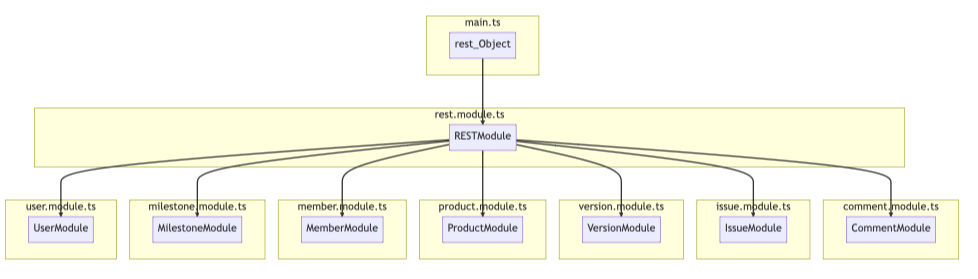
\includegraphics[width=1\textwidth]{backendmodules.png}
    \caption{Struktur der Module.tsx}
    \label{fig: backendmodules}
\end{figure}

Für jede Entität im Datenmodell ist im Verzeichnis ''packages/backend/src/modules/rest'' ist ein Ordner angelegt, welcher eine ''controller'', ''module'' und ''service'' Datei beinhaltet. In der ''module'' Datei wie zum Beispiel der product.module.ts wird definiert, welche Klassen die Aufgabe des Controllers, bzw. des Services übernehmen und welche Klassen importiert bzw. exportiert werden [siehe Abb. \ref{fig: moduleimport} auf S.~\pageref{fig: moduleimport}]. Die exportierte Klasse ''ProductModule'' wird, so wie die anderen Module der Endpunkte auch, in der ''rest.module.ts'' wieder importiert

\begin{figure}[h]
    \centering
    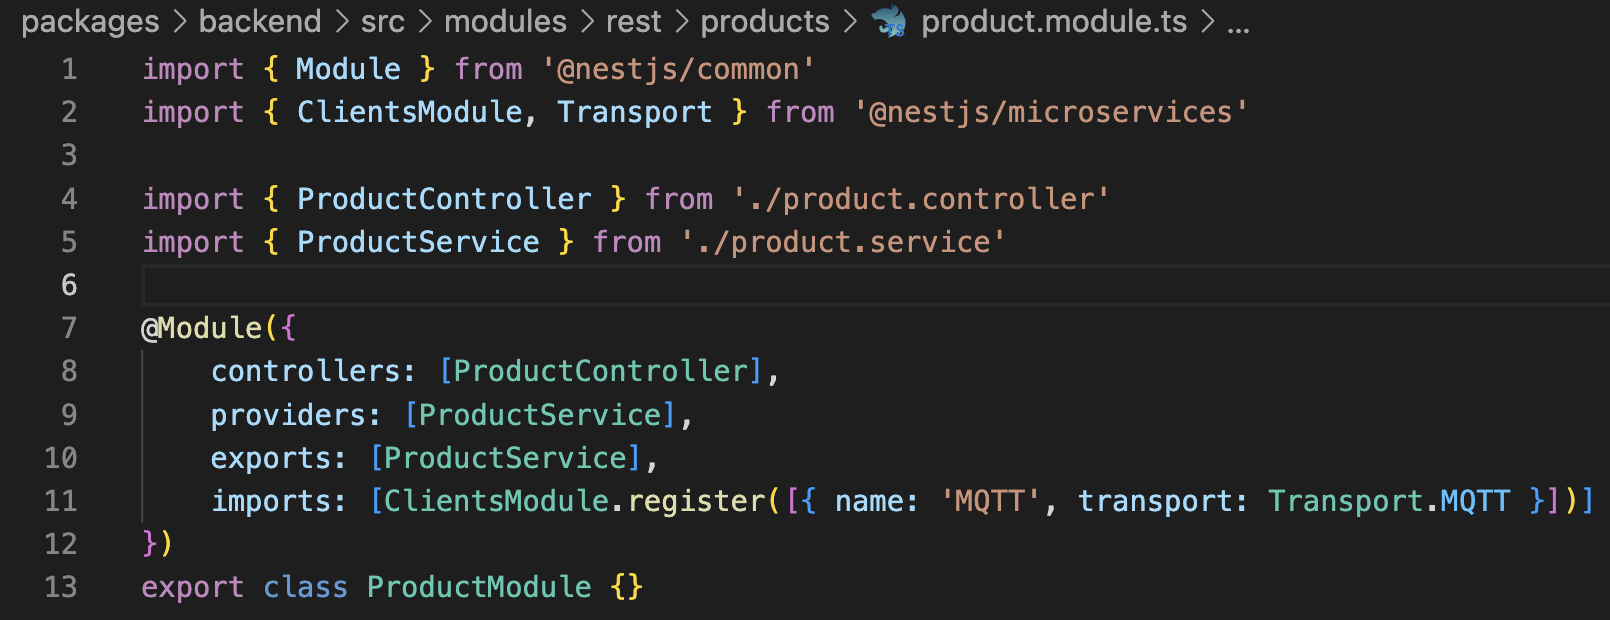
\includegraphics[width=1\textwidth]{moduleimport.png}
    \caption{Implementierung der product.module.ts}
    \label{fig: moduleimport}
\end{figure}

\section{Controller}
Der Controller hat die Aufgabe die eingehenden HTTP Requests zu empfangen und an den Service weiterzuleiten. Für die Durchführungen der ''CRUD'' Operationen werden folgende HTTP Methode verwendet:  ''Post'' um neue Daten an das Backend zu senden, ''Get'' um Daten aus dem Backend zu holen, ''Put'' um bestehende Daten zu verändern, ''Delete'' um Daten aus dem Backend zu löschen. Bevor der Controller den Service aufruft, wird noch geprüft, ob der aktuell eingeloggte User auch die Berechtigung hat die gewünschte Operation am Backend durchzuführen. Die Methoden zur Prüfung der Berechtigungen sind im der Datei ''permission.ts'' im Verzeichnis ''packages/backend/src/functions' implementiert. Diese Methoden werfen eine Exception, falls die nötigen Berechtigungen nicht vorhanden sind, und es kommt dadurch nicht dazu, dass der Controller den Service aufruft. Sind die Berechtigungen vorhanden, ruft der Controller, die im Service exportierte Funktion mit den möglichen Parametern der HTTP Nachricht auf. Dabei wird zwischen Parametern, die über den Query mitgesendet werden und Parameter, die als Body mitgesendet werden unterschieden. Als Beispiel ist als Abbildung ein ''PUT Request''. Als Query wird die ''id'' übertragen, um das gewünschte Produkt zu finden und als Body werden die neuen Daten übertragen um den Datensatz zu ändern [siehe Abb. \ref{fig: controllerput} auf S.~\pageref{fig: controllerput}]. Der Servicemethode werden die ''id'' und ''data'' mitgegeben.

\begin{figure}[h]
    \centering
    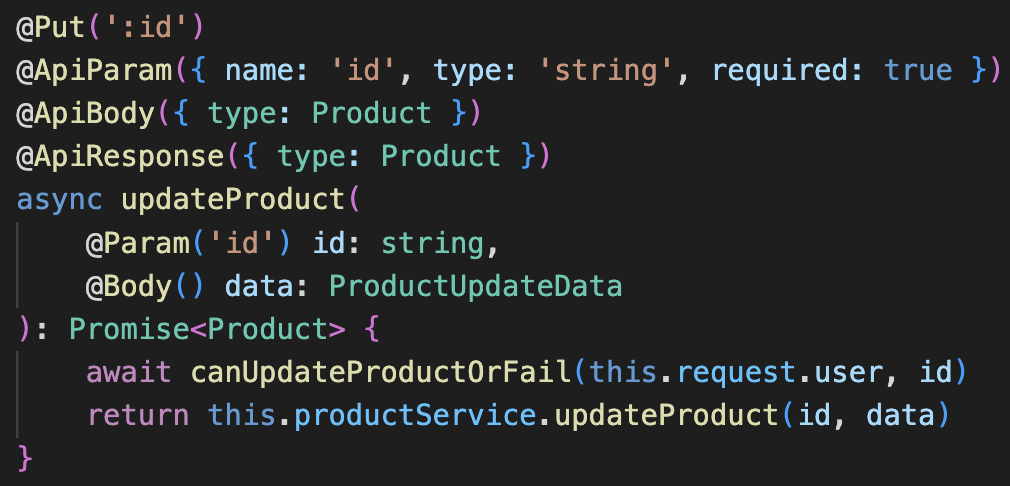
\includegraphics[width=1\textwidth]{controllerput.png}
    \caption{Implementierung von updateProduct im Controller}
    \label{fig: controllerput}
\end{figure}

\section{Service}
Im Service sind die Methoden implementiert, die die tatsächlichen Operationen auf den Daten ausführen. In der Abbildung [siehe Abb. \ref{fig: serviceput} auf S.~\pageref{fig: serviceput}]ist als Beispiel die ''updateProduct'' Methode aufgeführt. Diese Methode wird im Controller aufgerufen und es werden ihr die Parameter ''id'' und ''data'' übergeben. Als Erstes wird über die ''findOneByOrFail'' Methode zur gegebenen ''id'' ein passendes Produkt aus der Datenbank gesucht. Wird das Produkt gefunden wird es auf die Variable ''product'' geschrieben, wenn nicht, wird eine Exception geworfen. Im nächsten Schritt werden die Properties ''name'', ''description'' und ''public'' durch die Properties des übergebenen ''data'' Objektes überschrieben. Das veränderte Objekt wird mit der ''save'' Methode wieder in die Datenbank gespeichert. In der vorletzten Zeile wird eine MQTT Nachricht an das Frontend gesendet um mitzuteilen, dass der Cache nicht mehr aktuell ist, da sich ein Produkt geändert hat. Wenn das Frontend das nächste Mal nach den Produkten sucht, werden diese nicht mehr vom Cache zurückgegeben, sondern es wird ein Call ins Backend abgesetzt. Das Zusammenspiel aus Controller und Service erstreckt sich über alle Entitäten der Software und funktioniert immer nach diesem Prinzip. 

\begin{figure}[h]
    \centering
    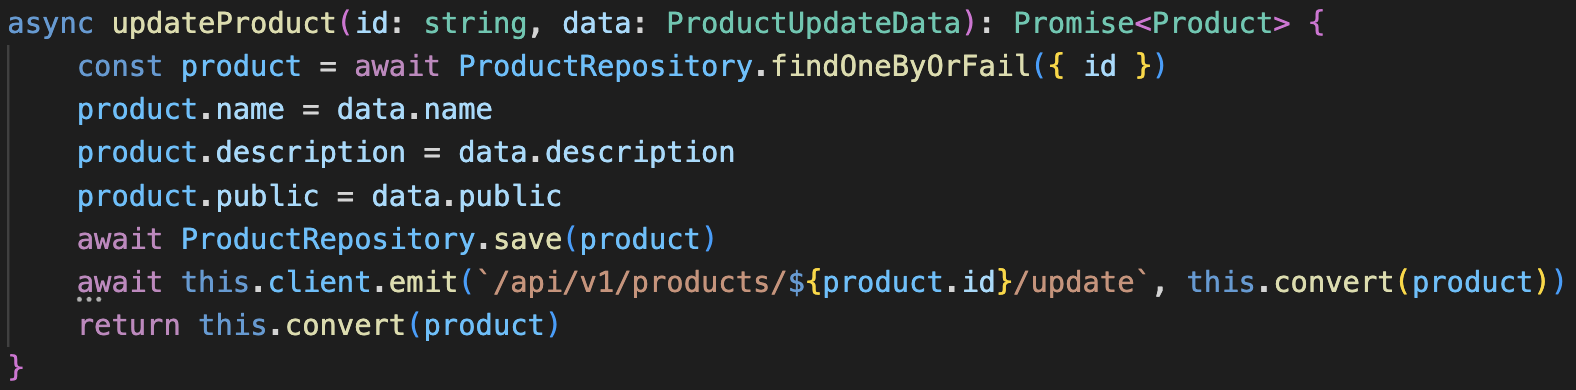
\includegraphics[width=1\textwidth]{serviceput.png}
    \caption{Implementierung von updateProduct im Service}
    \label{fig: serviceput}
\end{figure}


    %LTeX: language=de-DE
\chapter{Datenbank}
Für die Persistierung der Daten wird eine ''PostgreSQL\footnote{https://www.postgresql.org}'' Datenbank verwendet, die mithilfe von ''Docker\footnote{https://www.docker.com}'' in einem Container auf Port 5432 läuft. Die objektrelationale Abbildung der Objekte auf die Datenbank wird mit ''TypeORM\footnote{https://typeorm.io}'' durchgeführt.


\section{Main.ts}
Die Datei ''main.ts'' im Verzeichnis ''packages/database/src'' dient als Einstiegspunkt. Folgende Aufgaben werden hier ausgeführt:
\begin{itemize}
    \item Konfiguration, Erstellen und Export des Objektes ''AppDataSource''. Dieses Objekt wird später in der ''main.ts'' des Backends wieder importiert. ''AppDataSource'' ist dabei ein Objekt, das aus der Klasse ''DataSource'' gebaut wird welche aus dem ''TypeORM'' Modul stammt.
    \item Bauen der Repositories für jede Entität mit ''AppDataSource.getRepository()''. Die dafür nötigen Klassen der Entities werden aus dem ''entities'' Verzeichnis exportiert.
    \item Export der ''getEntityOrFail'' Methoden, welche in den ''Services'' im Backend verwendet werden.
\end{itemize}


\section{Entities}
Im Verzeichnis ''packages/database/src/entities'' liegt für jede Entity vom Datenmodell eine ''.ts'' Datei. In jeder dieser Dateien werden zuerst die nötigen Funktionen von ''TypeORM'' importiert. Danach folgt der Import der jeweiligen Entität aus dem ''Common'' Package. Weiters werden noch aus anderen Entitäten des ''entities'' Verzeichnisses jene Entities importiert, die in einer Beziehung zur aktuellen Entität stehen. Wie auch im Common Package und Backend Package wird auch hier viel mit ''Dekoratoren'' wie zum Beispiel ''@Entity'' gearbeitet, um dem darunterliegenden Code, Metadaten hinzuzufügen. Jedes Entity Klasse erbt von dem jeweiligen Import aus dem ''Common'' Package und ist mit ''@Entity'' ausgestattet, um eine Tabelle in der Datenbank zu repräsentieren. Für die Spalten werden ''@PrimaryColumn'' (PK) und @Column verwendet und mit ''ColumnOptions'' zusätzlich konfiguriert. So kann beispielsweise gesetzt werden, ob eine Spalte leer bleiben darf, einen Defaultvalue hat oder welche Zustande die Property haben kann wie zum Beispiel: ''enum: [manager, engineer, customer]''. Die Properties werden mit ''override name: datentyp'' angegeben. Mit ''@OneToMany'' bzw. ''@ManyToOne'' können 1:n bzw. n:1 Beziehungen zwischen den Tabellen definiert werden. Die nachfolgende Abbildung [siehe Abb. \ref{fig: dbentity} auf S.~\pageref{fig: dbentity}] zeigt, als Beispiel, die Implementierung der Entity ''Member''.

\begin{figure}[h]
    \centering
    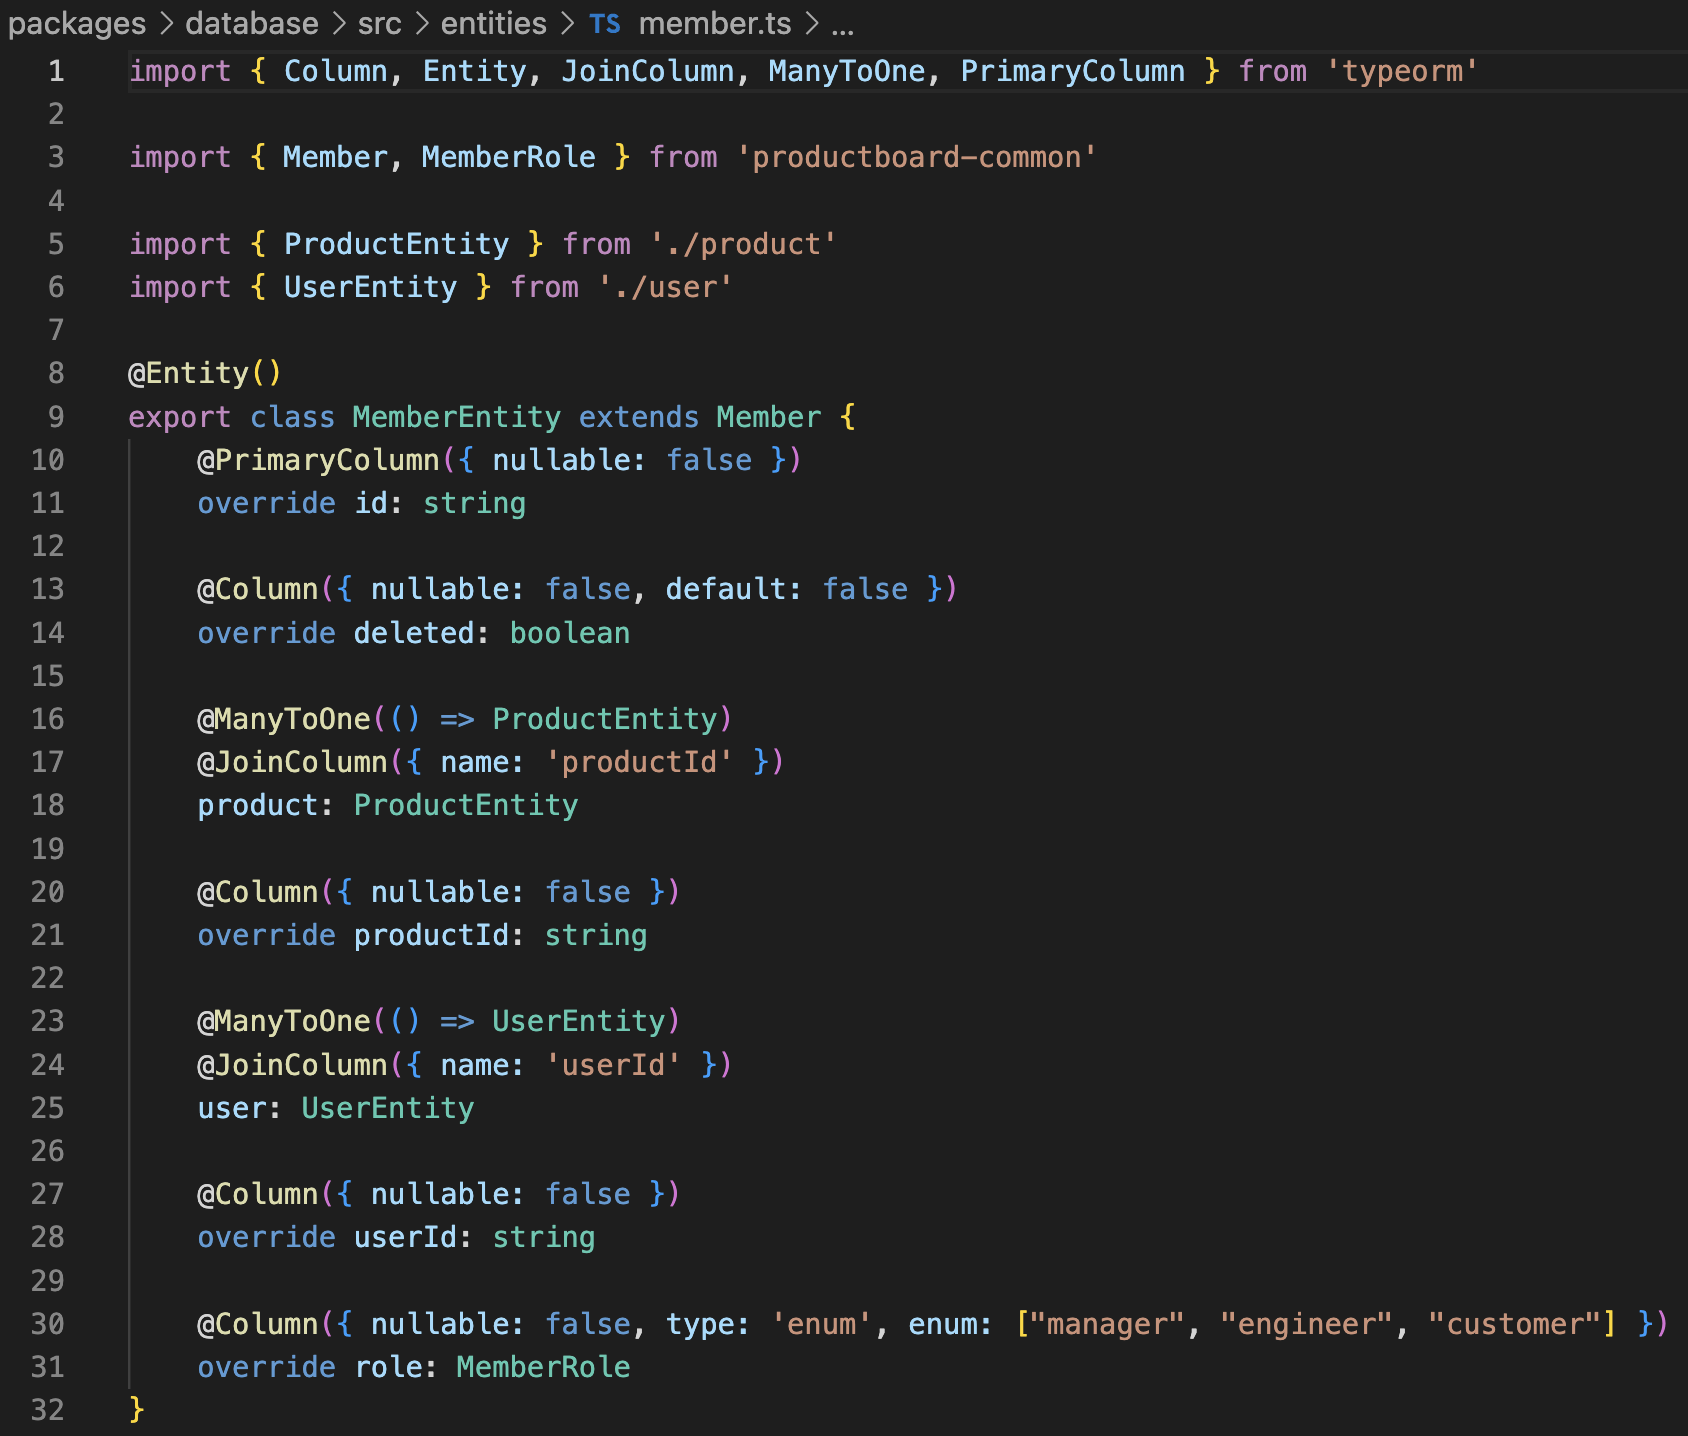
\includegraphics[width=1\textwidth]{dbentity.png}
    \caption{Member Entity.tsx}
    \label{fig: dbentity}
\end{figure}





    %% Zusammenfassung
    %\clearpage
    %LTeX: language=de-DE
\chapter{Zusammenfassung}
Bei dieser Software handelt es sich um eine ''Fullstack'' Webapplikation die komplett mit ''TypeScript'' erstellt wurde. In der nachfolgenden Liste sind zusammenfassend nochmal die wichtigsten Technologien aufgelistet, welche von dieser Applikation verwendet werden:

\begin{itemize}
    \item Übergreifend: TypeScript, Auth0, MQTT
    \item Gateway: Express
	\item Frontend: React.js, Axios, Three.js, Recharts
	\item Backend: Nest.js, Swagger, Postman
	\item Broker: Aedes,
	\item Datenbank: Docker, PostgreSQL, pgAdmin, TypeORM
\end{itemize}

Die Anwendung bietet noch eine Vielzahl von möglichen Funktionen, um die sie erweitert werden kann, wie beispielsweise:

\begin{itemize}
    \item Einbinden von Requirements Engineering
    \item Einbinden der Überführung von Requirements in eine CAD-feie Produktstruktur
    \item Das Verwalten von Produkten in verschiedensten Ausprägungen
    \item Einbauen von Simulationstools wie zum Beispiel ''FEM'' oder ''CFD''
    \item Prüfung der Qualität der CAD-Modelle anhand von Checklisten oder Meetings
    \item Umstellung von ''Three.js'' auf eine andere Engine für mehr Performance beim Rendern der Modelle
    \item Integration von verschiedensten Formaten oder Tools wie: PDF, Audio, Video, Simulationen oder CAD-Konstruktionstools für einen breiteren Einsatzbereich
\end{itemize}

Ein großer Vorteil dieses Projekts ist, dass durch die Anzahl an Technologien und durch die Abwechslung der Tätigkeiten viele neue Erkenntnisse gewonnen werden. Weiters werden nur modernste Technologien eingesetzt, die auch in der Wirtschaft breite Anwendung finden.

    %% Abbildungsverzeichnis
    \clearpage
    \renewcommand{\listfigurename}{Abbildungsverzeichnis}
\listoffigures
\label{sec: Abbildungen}
\chaptermark{\listfigurename}


    


%% Ende der ARBEIT
\end{document}